\documentclass[11pt]{article}
\usepackage{enumitem}
\usepackage{hyperref}
\hypersetup{
	colorlinks=true,
	linkcolor=blue,
	filecolor=magenta,      
	urlcolor=cyan,
}
\usepackage{graphicx}
\usepackage{amsmath}
\usepackage[utf8]{inputenc}
\usepackage{mathtools}
\usepackage[caption=false]{subfig}
\usepackage{soul}
\usepackage[top=0.75in, bottom=0.75in, left=0.5in, right=0.5in]{geometry}
\usepackage[margin=1.5cm]{caption}
\usepackage{epsfig,amsmath}
\DeclarePairedDelimiter\abs{${\lvert}$}{${\rvert}$}%
\usepackage{titlesec,color}
\usepackage{kpfonts}
\usepackage{empheq}
\usepackage{palatino}
\usepackage{graphicx,wrapfig}
\setlength{\parskip}{1em}
\setlength{\parindent}{0pt}
\usepackage{array}
\usepackage{gensymb}
\usepackage{soul}
\usepackage{grffile}
\usepackage{multicol}
\usepackage{listings}
\usepackage{color}
\usepackage{tcolorbox}
\usepackage{courier}
\usepackage[T1]{fontenc}
\usepackage{arial}
\usepackage{multicol}
\titleformat*{\section}{\small\bfseries}
\setlength\columnsep{0.3in}
\tcbuselibrary{listings,skins}
\tolerance=1
\emergencystretch=\maxdimen
\hyphenpenalty=10000
\hbadness=1000

\definecolor{dkgreen}{rgb}{0,0.6,0}
\definecolor{gray}{rgb}{0.5,0.5,0.5}
\definecolor{mauve}{rgb}{0.58,0,0.82}

\begin{document}
	
\renewcommand*\rmdefault{phv}
\fontfamily{phv}\selectfont
	
\cleardoublepage

\newpage
\begin{center}\textbf{Capital Bikeshare Program Data Report}\end{center}
\textbf{Summary}

Capital Bikeshare user data was used to construct a model to predict hourly usage (fig. 1). This model reveals several key predictors that could improve the ability of Capital Bikeshare to set prices, anticipate bike supply, and grow the bikeshare user base. Specifically, this shows that ride number depends heavily on the outdoor temperature and time of year. The model also suggests that over all usage of the bikeshare program is increasing on a year to year basis and that hourly demand follows two distinct usage patterns dependent on user type.

\begin{figure}[h!]
	\centering
	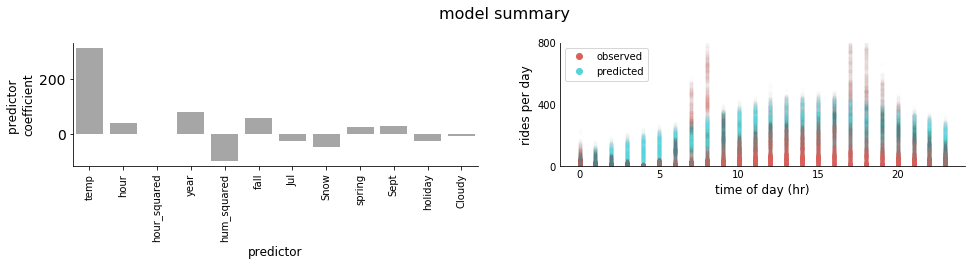
\includegraphics[width=0.97\textwidth]{figs/model_summary.png}
	\caption*{\footnotesize Figure 1. \textit{Left} Parameter coefficients for bikeshare usage model in order of predictive value. \textit{Right} Comparison of model predictions to actual bikeshare usage data.}
\end{figure}

\section{Lower prices in the winter and raise them in the summer}

Temperature was identified as the single best predictor of hourly usage (fig. 2). As expected, seasonal ride numbers are lowest in winter and highest in summer. For that reason, we recommend raising prices during the warmest months of the year when demand is high and lowering them during colder months. In particular, it may be worth reaching out to registered users to offer reduced fares during winter months.

\begin{figure}[h!]
	\centering
	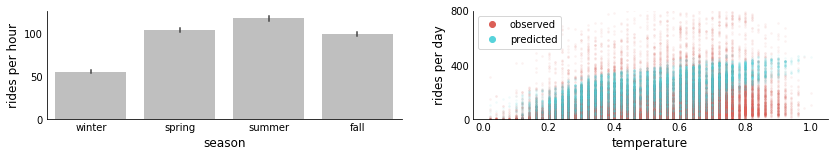
\includegraphics[width=0.97\textwidth]{figs/temp_effect.png}
	\caption*{\footnotesize Figure 2. \textit{Left} Bikeshare usage is much lower in winter than any other season. \textit{Right} Overlay of model predicted rides per day as a function of temperature. Temperature shows a strong positive effect on total usage.}
\end{figure}

\section{Offer lower fares for trips at non-peak hours}

We observed two distinct patterns of usage which might broadly correspond to work commutes and leisure trips (fig.3). Work commutes appear to be taken primarily by registered user and peak early in the morning at 9:00 and in the evening at 18:00. Leisure trips are taken primarily by casual users on work days and by both user types on weekends and holidays and appear to peak at 14:00. For this reason, we recommend offering reduced rates for non rush-hour times on work days and mornings and evenings on weekends and holidays.

\begin{figure}[h!]
	\centering
	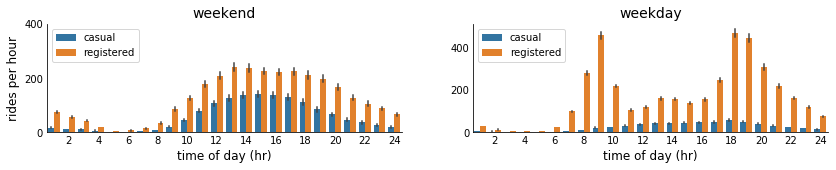
\includegraphics[width=0.97\textwidth]{figs/usertype_effect.png}
	\caption*{\footnotesize Figure 3. \textit{Left} Total usage on weekends peaks in the midday while \textit{Right} usage peaks in the morning and early evening in weekdays.}
\end{figure}


\section{Anticipate increased usage over the long term}

The Capital Bikeshare program grew rapidly between 2011 and 2012 and will continue to grow according to our model. For this reason, we recommend increasing the number of stations or the carrying capacity of existing stations in the program to meet growing demand in the following years.
 
\begin{figure}[h!]
	\centering
	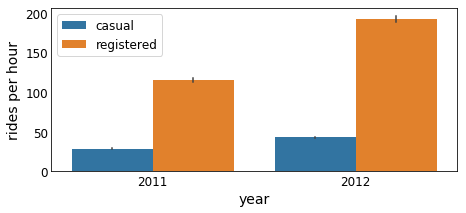
\includegraphics[width=0.4\textwidth]{figs/year_effect.png}
	\caption*{\footnotesize Figure 4. Average bike usage grew for both user types in between years 2011-2012}
\end{figure}

\end{document}